\documentclass{beamer}


% PACKAGES 
% ========
% Do not indent paragraphs and insert blank space between paragraphs.
\usepackage{parskip}

% To enter link, GitHub, and Twitter icons.
\usepackage{fontawesome}

% Commands like \textasciigrave, \textquotesingle, etc. are required by
% listings when \lstset{upquote=true} is used. They are defined in
% textcomp.sty.
\usepackage{textcomp}

% To enter syntax-highlighted code blocks.
\usepackage{listings}

% To perform absolute positioning of \faHandORight icon.
\usepackage{tikz}


% THEME
% =====
% Set main theme.
\usetheme{CambridgeUS}

% Set outer color theme.
\usecolortheme{seahorse}

% Set inner color theme for blocks.
\usecolortheme{orchid}

% Leave more margin from left and right side.
\setbeamersize{
    text margin left=1.5em,
    text margin right=1.5em,
}

% Align the frame title with the text with additional margin.
\setbeamertemplate{frametitle}[default][leftskip=0.5em]

% Remove navigation symbols from footer.
\setbeamertemplate{navigation symbols}{}

% CambridgeUS uses infolines.sty for outer theme which in turn defines
% footline with three color boxes for author, title, and date. We set
% the footline to omit the color box for title and distribute the width
% of the remaining two color boxes equally across the paper width. The
% code below is a derivative of the \defbeamertemplate*{footline} code
% in infolines.sty.
\setbeamertemplate{footline}
{%
  \leavevmode%
  \hbox{%
  \begin{beamercolorbox}[wd=.5\paperwidth,ht=2.25ex,dp=1ex,center]
        {author in head/foot}%
    \usebeamerfont{author in head/foot}\insertshortauthor
                  {~~~~(\insertshortinstitute)}
  \end{beamercolorbox}%
  \begin{beamercolorbox}[wd=.5\paperwidth,ht=2.25ex,dp=1ex,right]
        {date in head/foot}%
    \usebeamerfont{date in head/foot}\insertshortdate{}\hspace*{2em}
    \usebeamertemplate{page number in head/foot}\hspace*{2ex} 
  \end{beamercolorbox}}%
  \vskip0pt%
}


% IMAGES
% ======
% Image files search path.
\graphicspath{{img/}}


% CAPTIONS
% ========
% Customize caption font size and color.
\setbeamerfont{caption}{size=\scriptsize}
\setbeamercolor{caption name}{fg=black}

% Reduce vertical space around captions.
\setlength\abovecaptionskip{0pt}
\setlength\belowcaptionskip{0pt}

% Fake caption to show URL below screenshot and its caption.
% Font size of this fake caption should match that of beamer caption.
\newcommand{\linkcaption}[1]{
    \centering \scriptsize #1
}


% LINKS
% =====
% Color links blue.
\hypersetup{colorlinks=true,urlcolor=blue}

% Use current text font for links (override default teletype font).
\urlstyle{same}


% CODE LISTINGS
% =============
% Colors for syntax highlighting.
\definecolor{codecolor}{HTML}{000060} % dark blue
\definecolor{commentcolor}{HTML}{586e75} % bluish gray
\definecolor{keywordcolor}{HTML}{0000f0} % blue
\definecolor{stringcolor}{HTML}{600000} % dark red
\definecolor{placeholdercolor}{HTML}{006000} % dark green

% Base style for code listing.
\lstset{
    % Use small teletype font (override default roman font).
    basicstyle=\scriptsize\ttfamily\color{codecolor},
    % Use natural width of characters and do not mess with alignment.
    columns=fullflexible,
    % Do not drop consecutive spaces.
    keepspaces=true,
    % Use straight quotes instead of curved quotes.
    upquote=true,
    % Do not show spaces in strings as visible spaces.
    showstringspaces=false,
    % Set colors for syntax highlighting.
    commentstyle=\color{commentcolor},
    keywordstyle=\color{keywordcolor},
    stringstyle=\color{stringcolor},
}

% Plain code does not have any syntax highlighting.
\lstnewenvironment{plaincode}{}{}

% Content example code has only content headers highlighted.
\lstnewenvironment{contentcode}{
    \lstset{
        comment=[s]{<!--}{-->},
        commentstyle=\color{placeholdercolor},
    }
}{}

% Add HTML5 elements unrecognized by listings for highlighting.
% Highlight makesite template placeholders too.
\lstnewenvironment{htmlcode}{
    \lstset{
        language=html,
        morekeywords={main, footer},
        moredelim=[s][\color{placeholdercolor}]{\{\{}{\}\}},
    }
}{}

% Add Python keywords unrecognized by listings for highlighting.
\lstnewenvironment{pythoncode}{
    \lstset{
        language=python,
        morekeywords={yield, True, False},
    }
}{}

% Display inline code on a gray background.
\newcommand{\inlinecode}[1]{
    \colorbox{black!15}{%
        \texttt{#1}%
    }
}

% Title page information.
\title{Trending on Hacker News and GitHub \\ with 120 Lines of Python}
\subtitle{\vspace{2mm} From Writing to Publishing makesite.py}
\author{Sunaina Pai}
\institute[PyCon UK 2018, Cardiff, UK]{
    PyCon UK 2018, Cardiff City Hall, Cardiff, UK
}
\date{17 Sep 2018}


\begin{document}

% Title
\frame{\titlepage}

% who am i
\begin{frame}
    \frametitle{\texttt{who am i}}

    \textbf{Sunaina Pai}

    \bigskip

    Software Developer from Bangalore, India.

    Working with Java and big data technologies during the day.

    Exploring the beauty of Python and Lisp in the evening.

    \bigskip

    % Website
    \faLink{}
    \url{https://sunainapai.in/}

    % GitHub
    \faGithub{}
    \url{https://github.com/sunainapai}

    % Twitter
    \faTwitter{}
    \url{https://twitter.com/sunainapai}
\end{frame}


% Problem
\begin{frame}
    \frametitle{Problem}
    \begin{block}{Background}
    My static website/blog generator was written in shell script.
    \end{block}

    \bigskip

    \begin{block}{Problem}
    Write a new static site generator in a sane language!
    \end{block}

    \bigskip

    \begin{block}{Project}
    Write a few Python functions to render my static website/blog.
    \end{block}
\end{frame}


% Scope
\begin{frame}
    \frametitle{Scope}
    \begin{itemize}
        \item No magic!
        \item Minimal set of necessary features.
        \item Generate my website/blog with this project.
        \item Support multiple blogs in a website.
        \item Generate RSS feed for each blog.
        \item Share the project on Hacker News with a ``Show HN'' post.
    \end{itemize}
\end{frame}


% Directory Structure
\begin{frame}[fragile]
\frametitle{Directory Structure}
\begin{plaincode}
.
|-- makesite.py
|-- content
|   |-- _index.html
|   |-- about.html
|   |-- contact.html
|   |-- blog
|   |   |-- 2018-01-01-proin-quam.md
|   |   `-- 2018-01-03-sed-finibus.md
|   `-- news
|       |-- 2018-01-02-vivamus-purus.html
|       `-- 2018-01-04-mauris-tempor.html
|-- layout
|   |-- feed.xml
|   |-- item.html
|   |-- item.xml
|   |-- list.html
|   |-- page.html
|   `-- post.html
|-- static
|   `-- css
|       `-- style.css
`-- _site
\end{plaincode}
\end{frame}


% Layout Example
\begin{frame}[fragile]
\frametitle{Layout Template Example}
\begin{htmlcode}
<!DOCTYPE html>
<html>
  <head>
    <title>{{ title }} - {{ subtitle }}</title>
    <meta charset="UTF-8">
    <meta name="viewport" content="width=device-width">
    <link rel="stylesheet" type="text/css" href="/css/style.css">
  </head>
  <body>
    <main>
      {{ content }}
    </main>
    <footer>
      <div>&copy; {{ current_year }} Lorem Ipsum</div>
    </footer>
  </body>
</html>
\end{htmlcode}
\end{frame}


% Content Example
\begin{frame}[fragile]
\frametitle{Content Example}
\begin{contentcode}
<!-- title: Proin Quam -->
<!-- author: Alice -->
Proin quam urna, pulvinar id ipsum ac, mattis consectetur ante. Praesent
non justo lectus. Duis egestas arcu libero, quis laoreet dolor volutpat
ut. Donec facilisis orci sit amet sem blandit elementum.

Vestibulum suscipit consectetur diam, ac posuere metus condimentum in.
Integer vehicula vitae enim id gravida.

Vestibulum ut eros vitae risus porttitor porta in eget felis. Nulla
lorem erat, mattis eget lacus eget, interdum aliquet lectus. Fusce non
felis diam.
\end{contentcode}
\end{frame}


% Code Walkthrough: Source Code URL
\begin{frame}
\frametitle{Code Walkthrough: Source Code URL}
\centering

\href{https://git.io/makesite.py}{%
    
\includegraphics[width=1.75in]{makesite-py-qr.png}%
}

\medskip

\Huge \href{https://git.io/makesite.py}{git.io/makesite.py}
\end{frame}


% Code Walkthrough: Utilities: fread(), fwrite()
\begin{frame}[fragile]
\frametitle{Code Walkthrough: Utilities}
\begin{pythoncode}
import os
import shutil
import re
import glob
import sys
import json
import datetime

def fread(filename):
    """Read file and close the file."""
    with open(filename, 'r') as f:
        return f.read()


def fwrite(filename, text):
    """Write content to file and close the file."""
    basedir = os.path.dirname(filename)
    if not os.path.isdir(basedir):
        os.makedirs(basedir)

    with open(filename, 'w') as f:
        f.write(text)
\end{pythoncode}
\end{frame}


% Code Walkthrough: Utilities: log(), truncate(), rfc_2822_format()
\begin{frame}[fragile]
\frametitle{Code Walkthrough: Utilities}
\begin{pythoncode}
def log(msg, *args):
    """Log message with specified arguments."""
    sys.stderr.write(msg.format(*args) + '\n')


def truncate(text, words=25):
    """Remove tags and truncate text to the specified number of words."""
    return ' '.join(re.sub('(?s)<.*?>', ' ', text).split()[:words])


def rfc_2822_format(date_str):
    """Convert yyyy-mm-dd date string to RFC 2822 format date string."""
    d = datetime.datetime.strptime(date_str, '%Y-%m-%d')
    return d.strftime('%a, %d %b %Y %H:%M:%S +0000')
\end{pythoncode}
\end{frame}


% Code Walkthrough: Header Parsing: read_headers()
\begin{frame}[fragile]
\frametitle{Code Walkthrough: Header Parsing}
\begin{pythoncode}
def read_headers(text):
    """Parse headers in text and yield (key, value, end-index) tuples."""
    for match in re.finditer('\s*<!--\s*(.+?)\s*:\s*(.+?)\s*-->\s*|.+', text):
        if not match.group(1):
            break
        yield match.group(1), match.group(2), match.end()
\end{pythoncode}

\begin{block}{A note on headers}
Headers are key-value pairs within HTML comments at the top of a content
file.

\medskip

\begin{contentcode}
<!-- title: Proin Quam -->
<!-- author: Alice -->
<!-- key1: value1 -->
<!-- key2: value2 -->
Content
\end{contentcode}
\end{block}
\end{frame}


% Code Walkthrough: Content Parsing: read_content(): 1/2
\begin{frame}[fragile]
\frametitle{Code Walkthrough: Content Parsing}
\begin{pythoncode}
def read_content(filename):
    """Read content and metadata from file into a dictionary."""
    # Read file content.
    text = fread(filename)

    # Read metadata and save it in a dictionary.
    date_slug = os.path.basename(filename).split('.')[0]
    match = re.search('^(?:(\d\d\d\d-\d\d-\d\d)-)?(.+)$', date_slug)
    content = {
        'date': match.group(1) or '1970-01-01',
        'slug': match.group(2),
    }

    # Read headers.
    end = 0
    for key, val, end in read_headers(text):
        content[key] = val

    # Separate content from headers.
    text = text[end:]

    # ... read_content() definition continued on next slide ...
\end{pythoncode}
\end{frame}


% Code Walkthrough: Content Parsing: read_content(): 2/2
\begin{frame}[fragile]
\frametitle{Code Walkthrough: Content Parsing}
\begin{pythoncode}
    # ... read_content() definition continued from previous slide ... 

    # Convert Markdown content to HTML.
    if filename.endswith(('.md', '.mkd', '.mkdn', '.mdown', '.markdown')):
        try:
            if _test == 'ImportError':
                raise ImportError('Error forced by test')
            import CommonMark
            text = CommonMark.commonmark(text)
        except ImportError as e:
            log('WARNING: Cannot render Markdown in {}: {}', filename, str(e))

    # Update the dictionary with content and RFC 2822 date.
    content.update({
        'content': text,
        'rfc_2822_date': rfc_2822_format(content['date'])
    })

    return content
\end{pythoncode}
\end{frame}


% Code Walkthrough: Template Rendering: render()
\begin{frame}[fragile]
\frametitle{Code Walkthrough: Template Rendering}
\begin{pythoncode}
def render(template, **params):
    """Replace placeholders in template with values from params."""
    return re.sub(r'{{\s*([^}\s]+)\s*}}',
                  lambda match: str(params.get(match.group(1), match.group(0))),
                  template)
\end{pythoncode}

\vspace{-0.35em}

\begin{block}{A note on rendering}
Key-values represented by \inlinecode{**params} populate placeholders with
matching names in templates. For example, if \inlinecode{template} is

\begin{htmlcode}
<head><title>{{ title }} - {{ subtitle }}</title></head>
<body>{{ content }}</body>
\end{htmlcode}

then

\begin{pythoncode}
render(template, title='About', subtitle='Lorem Ipsum', content='Foo')
\end{pythoncode}

returns

\begin{htmlcode}
<head><title>About - Lorem Ipsum</title></head>
<body><p>Foo</p></body>
\end{htmlcode}
\end{block}
\end{frame}


% Code Walkthrough: Building Blocks: make_pages()
\begin{frame}[fragile]
\frametitle{Code Walkthrough: Building Blocks}
\begin{pythoncode}
def make_pages(src, dst, layout, **params):
    """Generate pages from page content."""
    items = []

    for src_path in glob.glob(src):
        content = read_content(src_path)
        page_params = dict(params, **content) 

        # Populate placeholders in content if content-rendering is enabled.
        if page_params.get('render') == 'yes':
            rendered_content = render(page_params['content'], **page_params)
            page_params['content'] = rendered_content
            content['content'] = rendered_content

        items.append(content)

        dst_path = render(dst, **page_params)
        output = render(layout, **page_params)

        log('Rendering {} => {} ...', src_path, dst_path)
        fwrite(dst_path, output)

    return sorted(items, key=lambda x: x['date'], reverse=True)
\end{pythoncode}
\end{frame}


% Code Walkthrough: Building Blocks: make_list()
\begin{frame}[fragile]
\frametitle{Code Walkthrough: Building Blocks}
\begin{pythoncode}
def make_list(posts, dst, list_layout, item_layout, **params):
    """Generate list page for a blog."""
    items = []
    for post in posts:
        item_params = dict(params, **post)
        item_params['summary'] = truncate(post['content'])
        item = render(item_layout, **item_params)
        items.append(item)

    params['content'] = ''.join(items)
    dst_path = render(dst, **params)
    output = render(list_layout, **params)

    log('Rendering list => {} ...', dst_path)
    fwrite(dst_path, output)
\end{pythoncode}
\end{frame}


% Code Walkthrough: Tying It All Together: main(): 1/4
\begin{frame}[fragile]
\frametitle{Code Walkthrough: Tying It All Together}
\begin{pythoncode}
def main():
    # Create a new _site directory from scratch.
    if os.path.isdir('_site'):
        shutil.rmtree('_site')
    shutil.copytree('static', '_site')

    # Default parameters.
    params = {
        'base_path': '',
        'subtitle': 'Lorem Ipsum',
        'author': 'Admin',
        'site_url': 'http://localhost:8000',
        'current_year': datetime.datetime.now().year
    }

    # If params.json exists, load it.
    if os.path.isfile('params.json'):
        params.update(json.loads(fread('params.json')))

    # ... main() definition continued on next slide ...
\end{pythoncode}
\end{frame}


% Code Walkthrough: Tying It All Together: main(): 2/4
\begin{frame}[fragile]
\frametitle{Code Walkthrough: Tying It All Together}
\begin{pythoncode}
    # ... main() definition continued from previous slide ...

    # Load layouts.
    page_layout = fread('layout/page.html')
    post_layout = fread('layout/post.html')
    list_layout = fread('layout/list.html')
    item_layout = fread('layout/item.html')
    feed_xml = fread('layout/feed.xml')
    item_xml = fread('layout/item.xml')

    # Combine layouts to form final layouts.
    post_layout = render(page_layout, content=post_layout)
    list_layout = render(page_layout, content=list_layout)

    # Create site pages.
    make_pages('content/_index.html', '_site/index.html',
               page_layout, **params)
    make_pages('content/[!_]*.html', '_site/{{ slug }}/index.html',
               page_layout, **params)

    # ... main() definition continued on next slide ...
\end{pythoncode}
\end{frame}


% Code Walkthrough: Tying It All Together: main(): 3/4
\begin{frame}[fragile]
\frametitle{Code Walkthrough: Tying It All Together}
\begin{pythoncode}
    # ... main() definition continued from previous slide ...

    # Create blogs.
    blog_posts = make_pages('content/blog/*.md',
                            '_site/blog/{{ slug }}/index.html',
                            post_layout, blog='blog', **params)
    news_posts = make_pages('content/news/*.html',
                            '_site/news/{{ slug }}/index.html',
                            post_layout, blog='news', **params)

    # Create blog list pages.
    make_list(blog_posts, '_site/blog/index.html',
              list_layout, item_layout, blog='blog', title='Blog', **params)
    make_list(news_posts, '_site/news/index.html',
              list_layout, item_layout, blog='news', title='News', **params)

    # Create RSS feeds.
    make_list(blog_posts, '_site/blog/rss.xml',
              feed_xml, item_xml, blog='blog', title='Blog', **params)
    make_list(news_posts, '_site/news/rss.xml',
              feed_xml, item_xml, blog='news', title='News', **params)
\end{pythoncode}
\end{frame}


% Code Walkthrough: Tying It All Together: ./makesite.py: 4/4
\begin{frame}[fragile]
\frametitle{Code Walkthrough: Tying It All Together}
\begin{pythoncode}
# Test parameter to be set temporarily by unit tests.
_test = None

if __name__ == '__main__':
    main()
\end{pythoncode}

    \begin{block}{Generating Static Website/Blog}
        Running \inlinecode{./makesite.py} generates the static
        website/blog and writes it to \inlinecode{\_site} directory.
    \end{block}

    \begin{block}{Local Testing}
        The project comes with a convenience {{make serve}} target to
        generate the static website/blog and serve it locally with
        \inlinecode{SimpleHTTPServer} or \inlinecode{http.server}
        (Python 3) on port 8000.
    \end{block}

\end{frame}


% Project URLs
\begin{frame}[fragile]
    \frametitle{Project URLs}
    Source code: \url{https://github.com/sunainapai/makesite}

    Short URL: \url{https://git.io/makesite}

    \bigskip

    Demo website/blog: \url{https://tmug.github.io/makesite-demo/}

    Short URL: \url{https://git.io/makesite-demo}

    \bigskip

\begin{block}{Creating Short URLs}
\begin{plaincode}
curl -i https://git.io \
     -F "url=https://github.com/sunainapai/makesite" \
     -F "code=makesite"

curl -i https://git.io \
     -F "url=https://tmug.github.io/makesite-demo/" \
     -F "code=makesite-demo"
\end{plaincode}
\end{block}
\end{frame}


% On Hacker News (Screenshot)
\begin{frame}
    \frametitle{On Hacker News}

    \begin{figure}
        \centering
        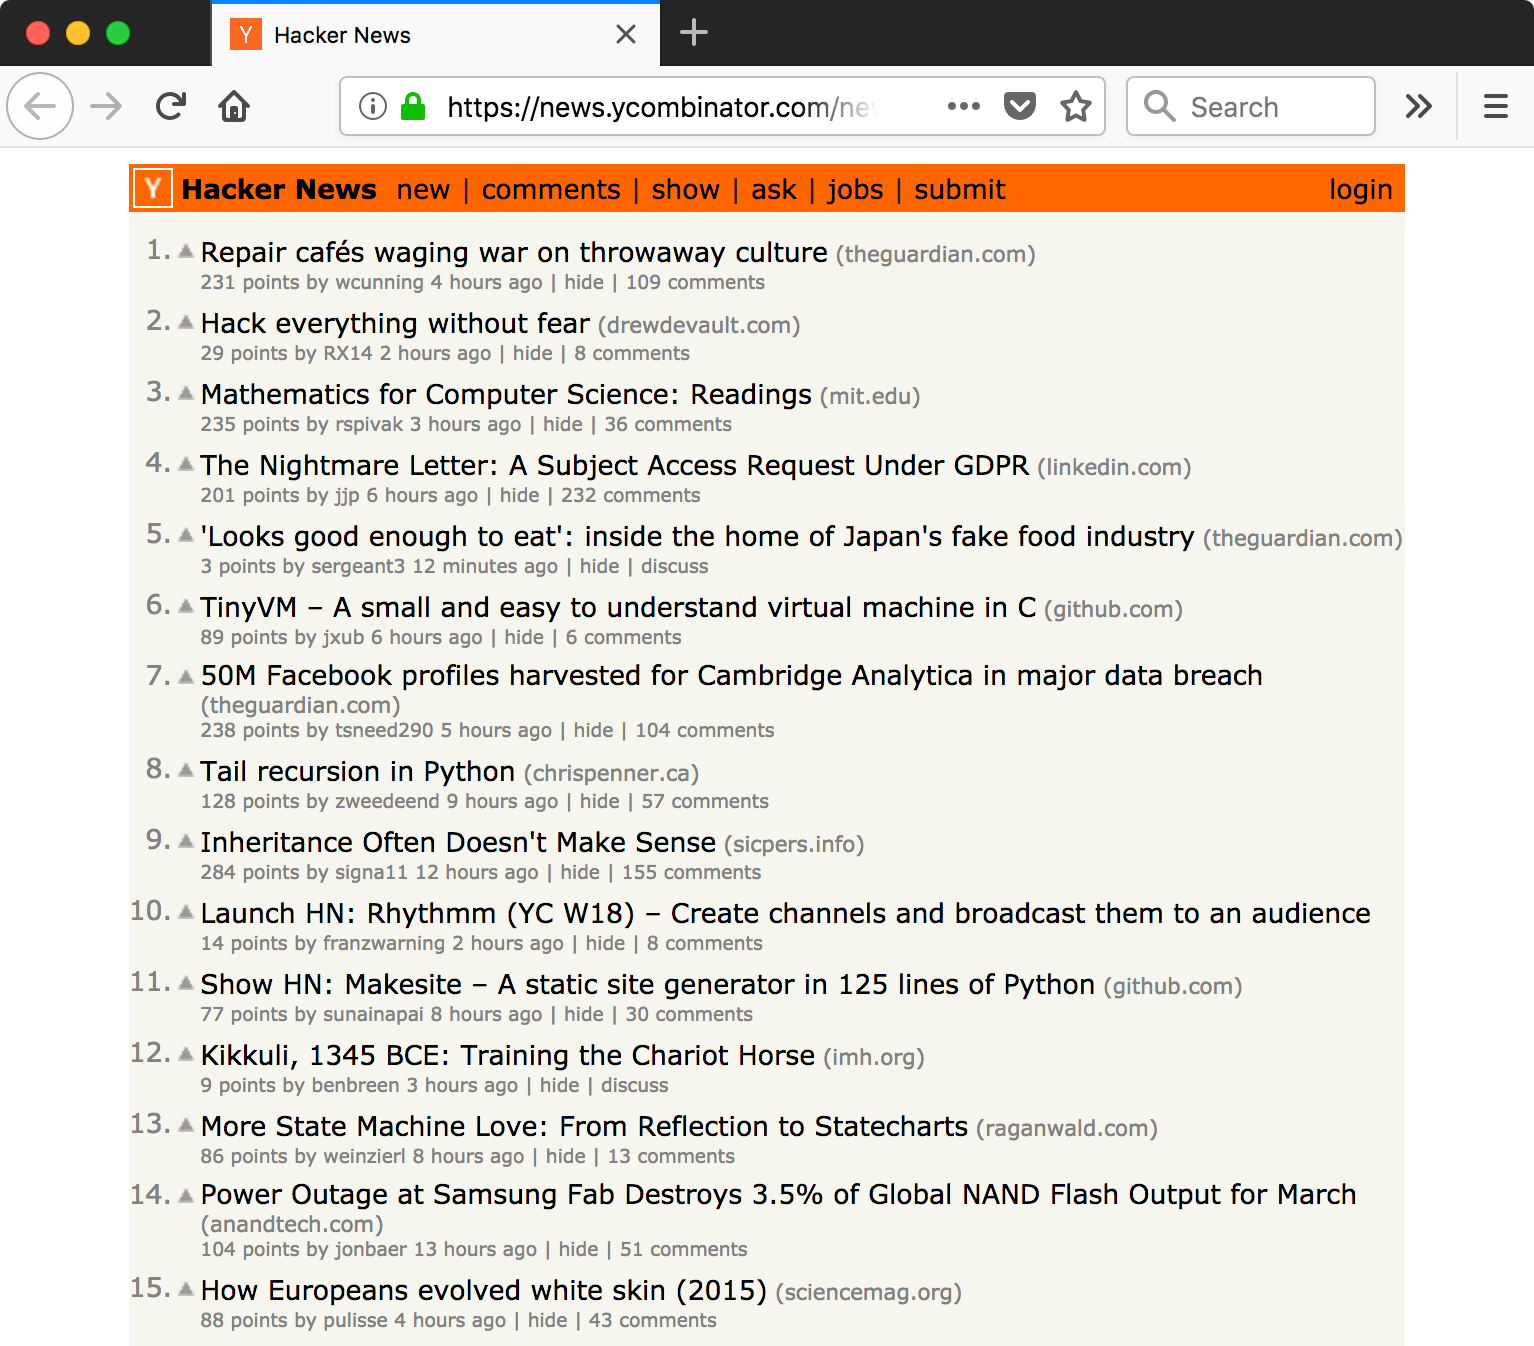
\includegraphics[height=2.4in]{makesite-hn.png}
        \caption{
            Makesite trending on the Hacker News front page on 17 Mar 2018
        }
    \end{figure}

    \linkcaption{
        Hacker News ``Show HN'' story:
        \url{https://news.ycombinator.com/item?id=16606408}
    }

    \begin{tikzpicture}[remember picture, overlay]
        \node [xshift=32.4mm, yshift=36mm] at (current page.south west) {
            \footnotesize \faHandORight
        };
    \end{tikzpicture}
\end{frame}


% GitHub Repository (Screenshot)
\begin{frame}
    \frametitle{GitHub Repository}

    \begin{figure}
        \centering
        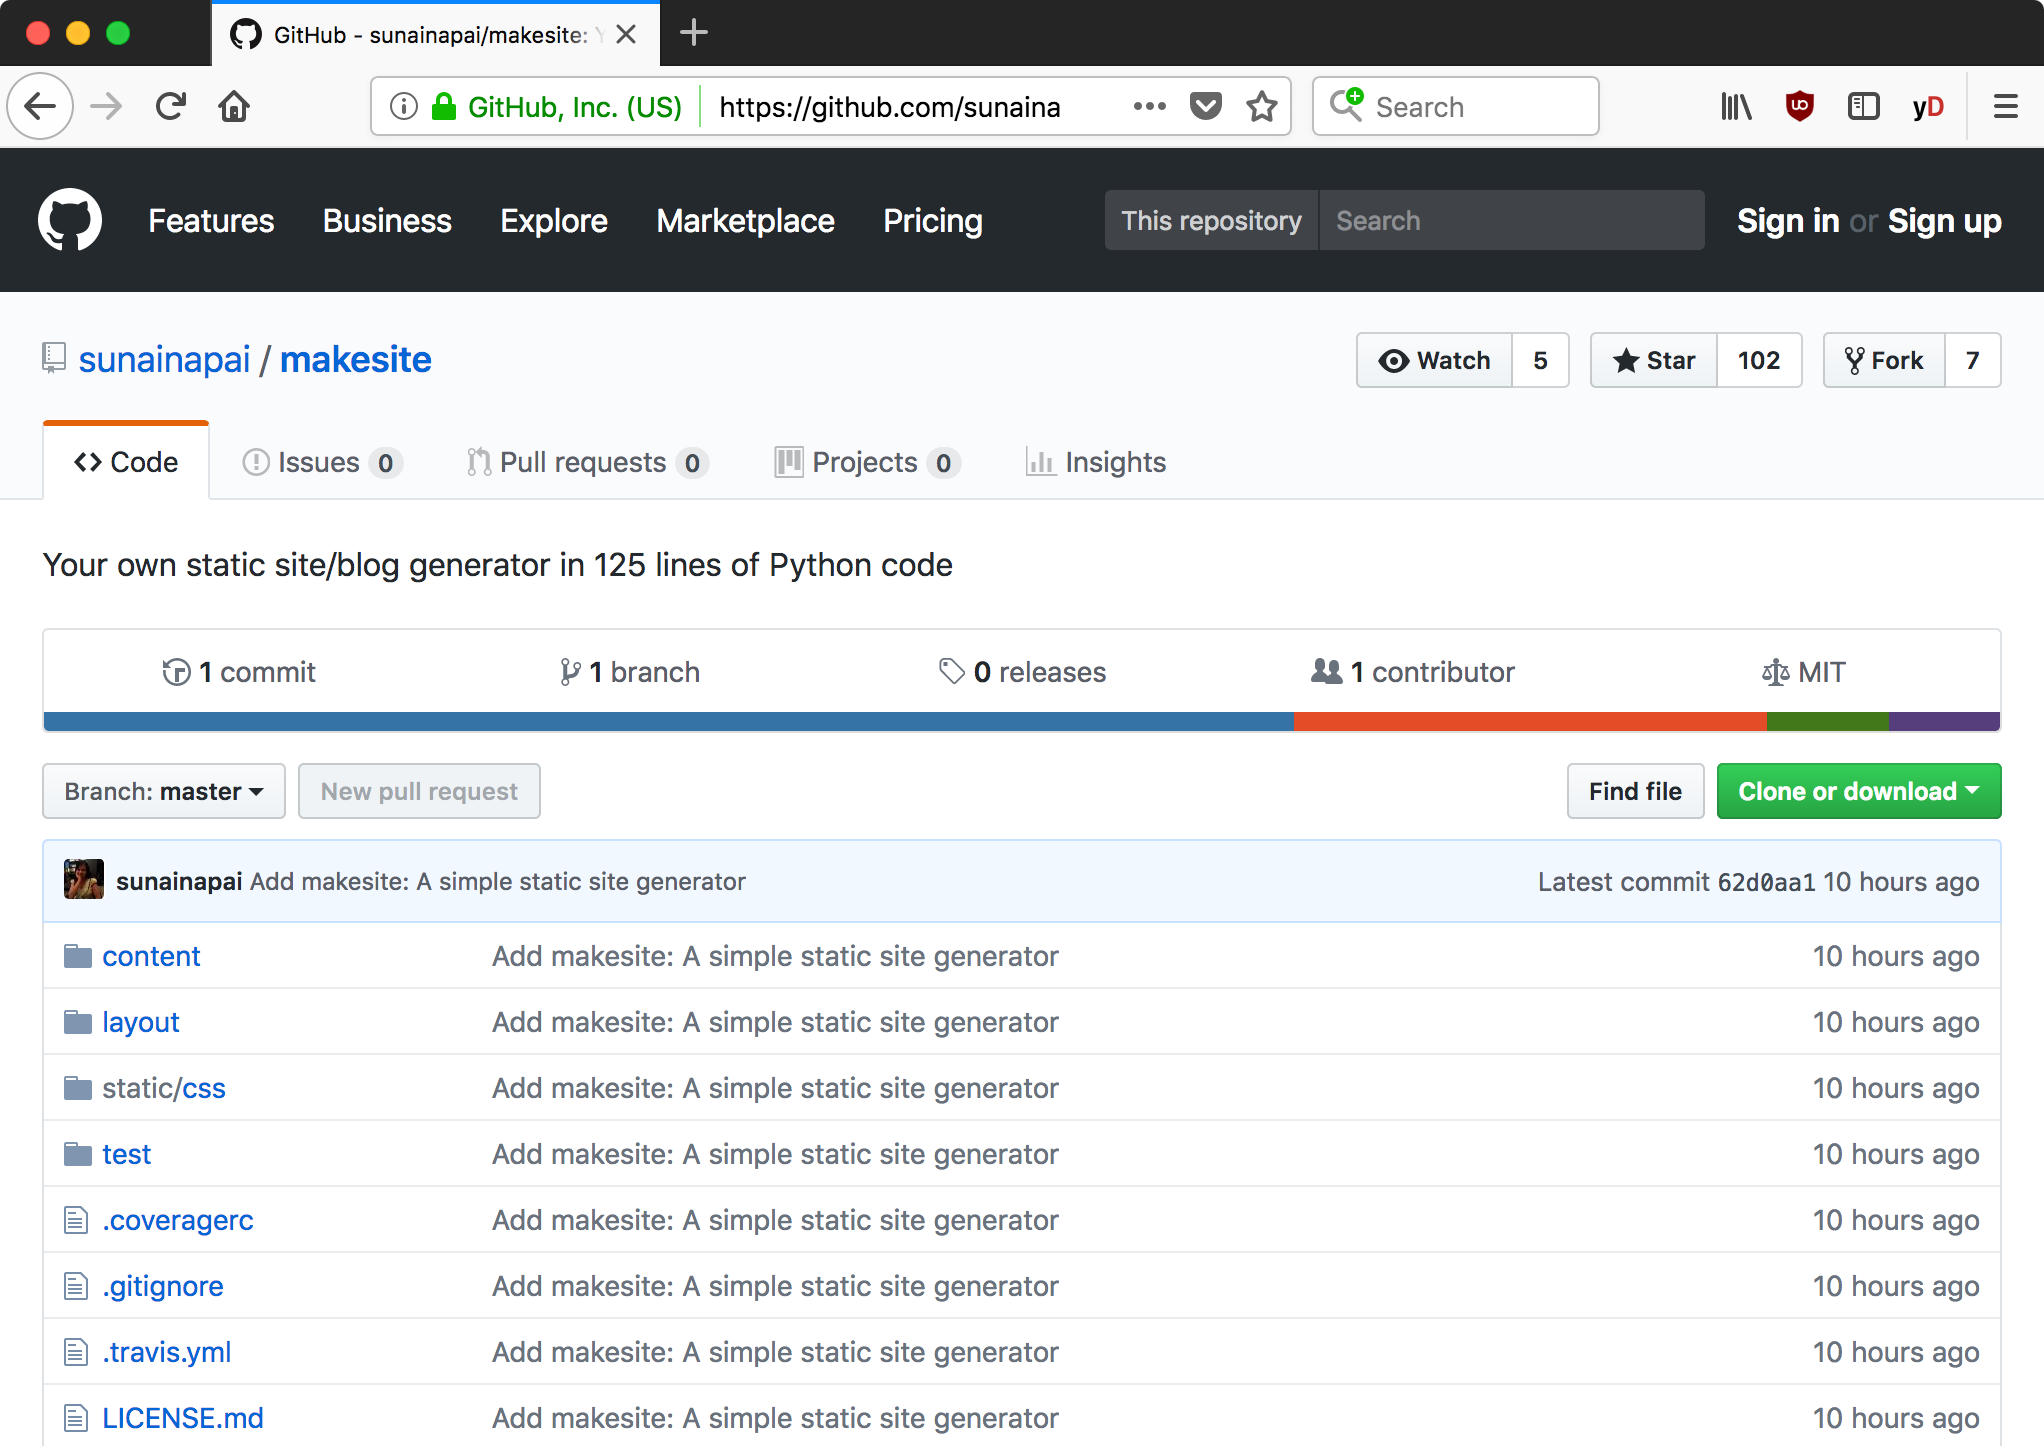
\includegraphics[height=2.4in]{makesite-github.png}
        \caption{Screenshot of GitHub repository taken on 17 Mar 2018}
    \end{figure}

    \linkcaption{
        GitHub repository: \url{https://github.com/sunainapai/makesite}
    }
\end{frame}


% Project README (Screenshot)
\begin{frame}
    \frametitle{Project README}

    \begin{figure}
        \centering
        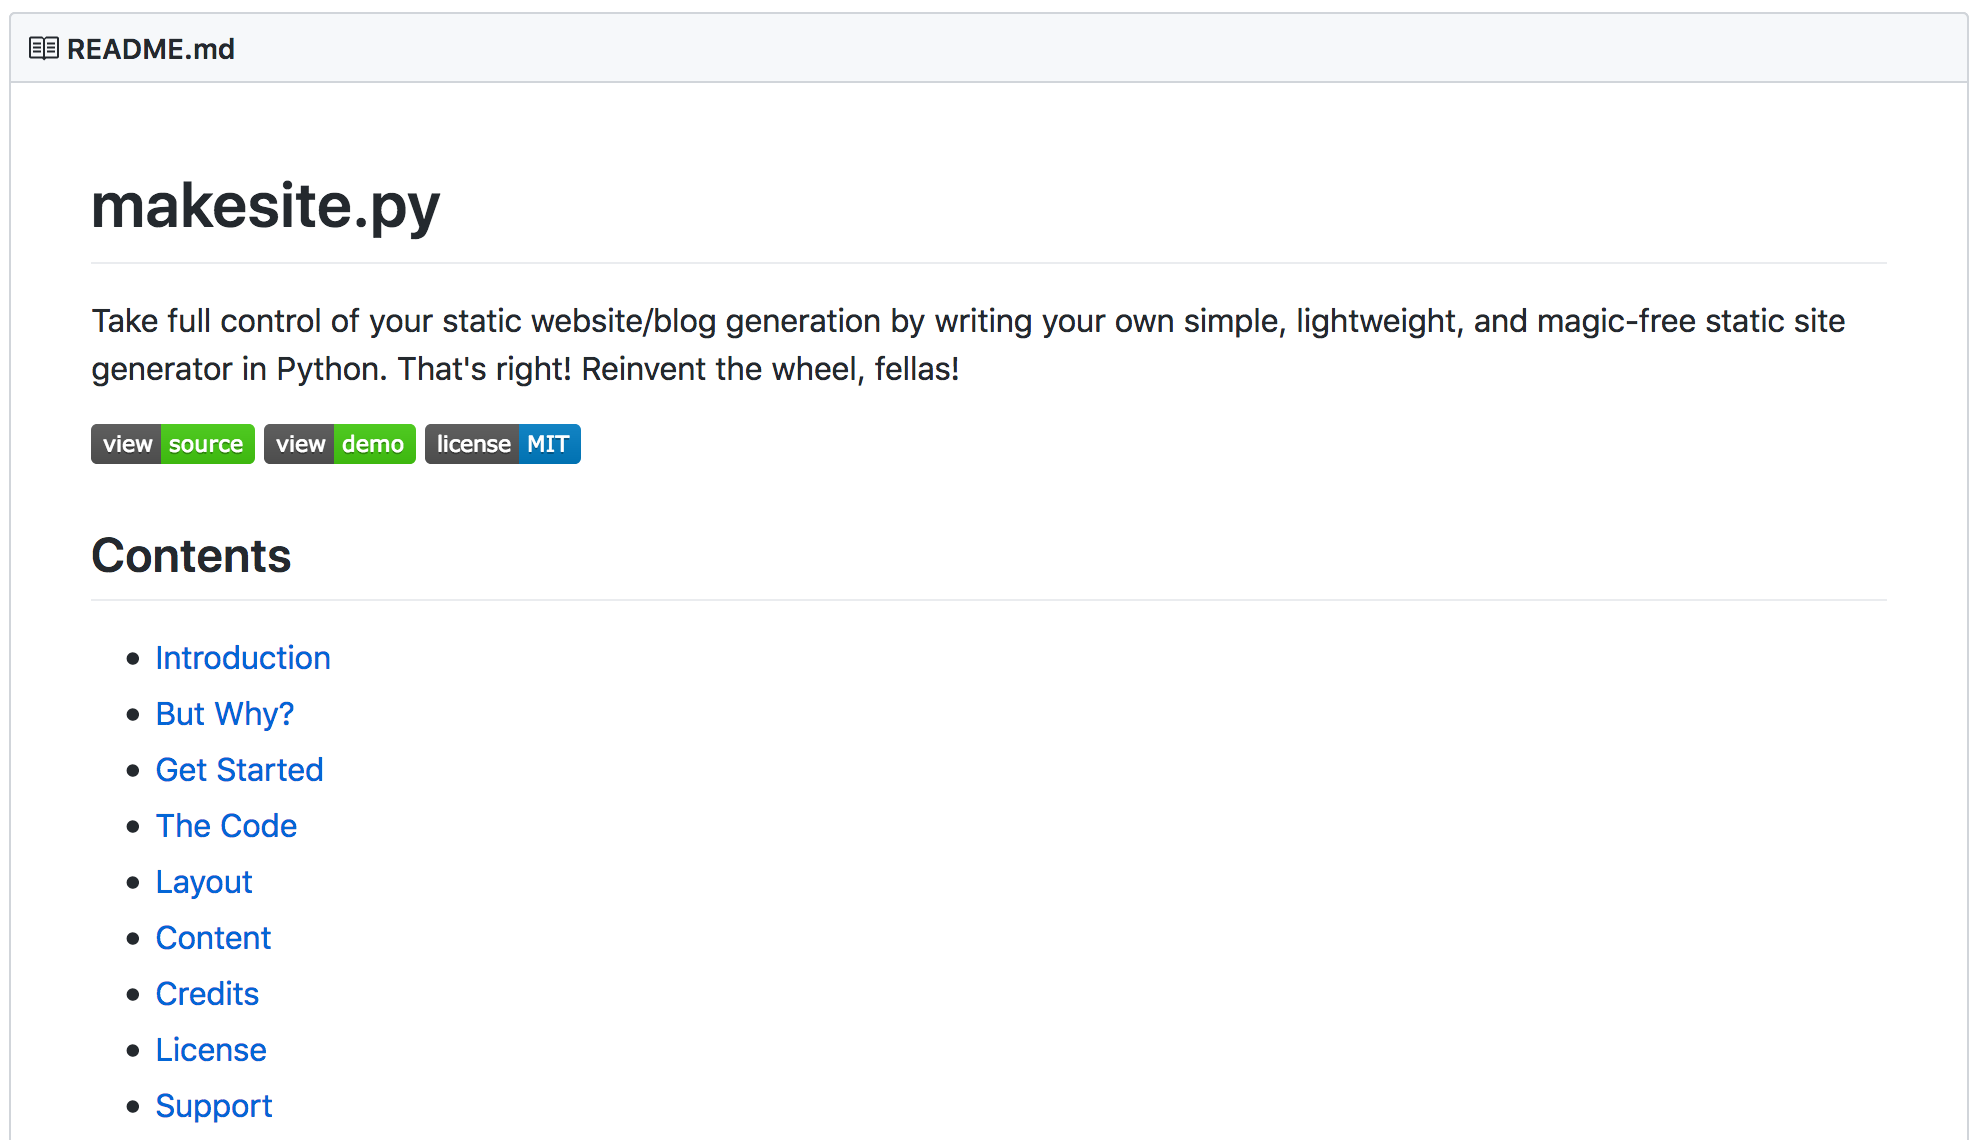
\includegraphics[height=2.4in]{makesite-readme.png}
        \caption{Screenshot of project README}
    \end{figure}

    \linkcaption{
        GitHub repository: \url{https://github.com/sunainapai/makesite}
    }
\end{frame}


% Travis CI and Coveralls Integration
\begin{frame}
    \frametitle{Travis CI and Coveralls Integration}

    \begin{figure}
        \centering
        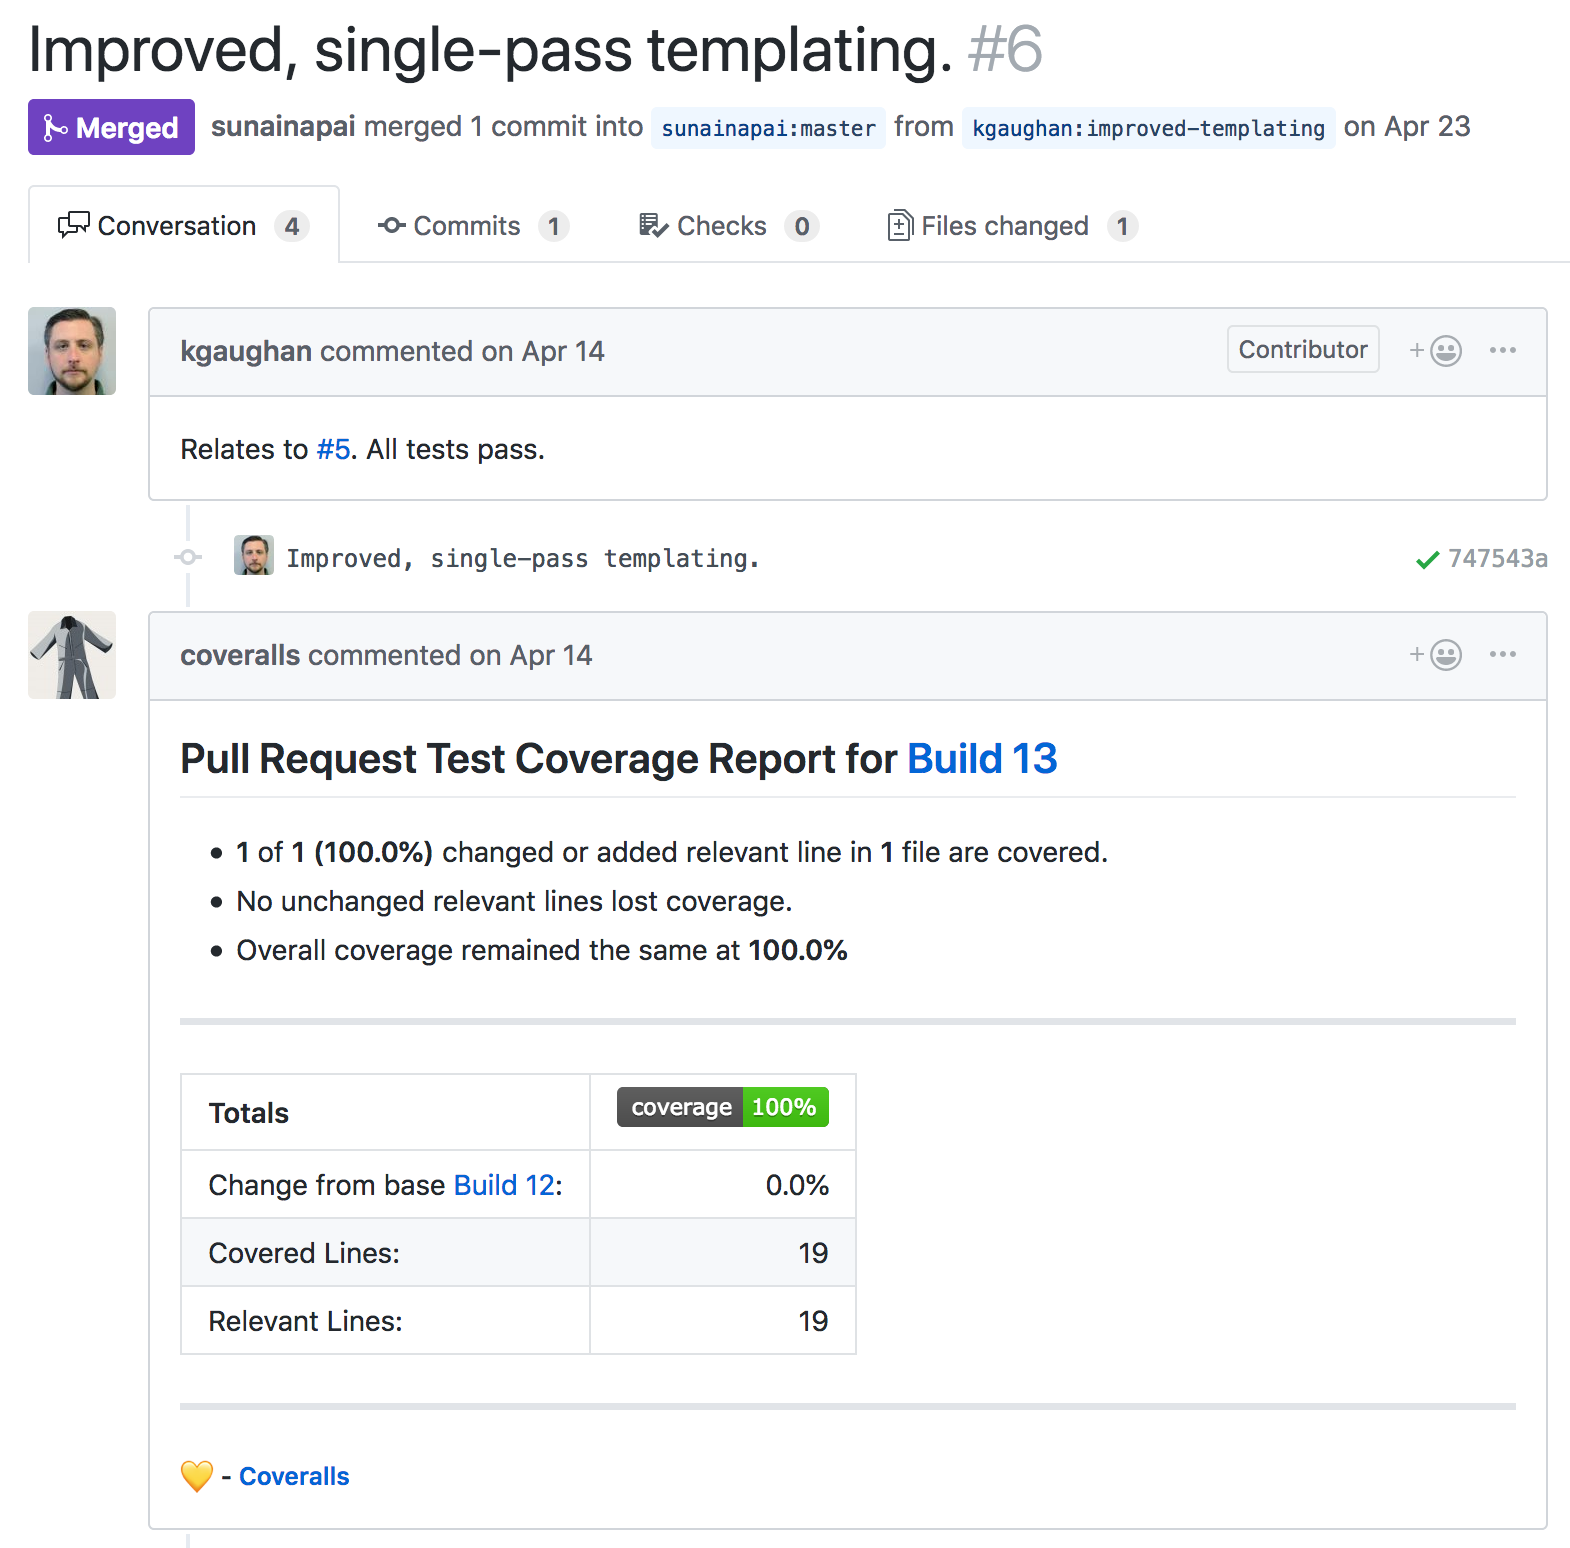
\includegraphics[height=2.4in]{makesite-coverage.png}
        \caption{Unit testing and coverage for pull requests and commits}
    \end{figure}

    \linkcaption{
        Pull Request URL: \url{https://github.com/sunainapai/makesite/pull/6}
    }
\end{frame}


% Demo Static Website (Screenshot)
\begin{frame}
    \frametitle{Demo Static Website}

    \begin{figure}
        \centering
        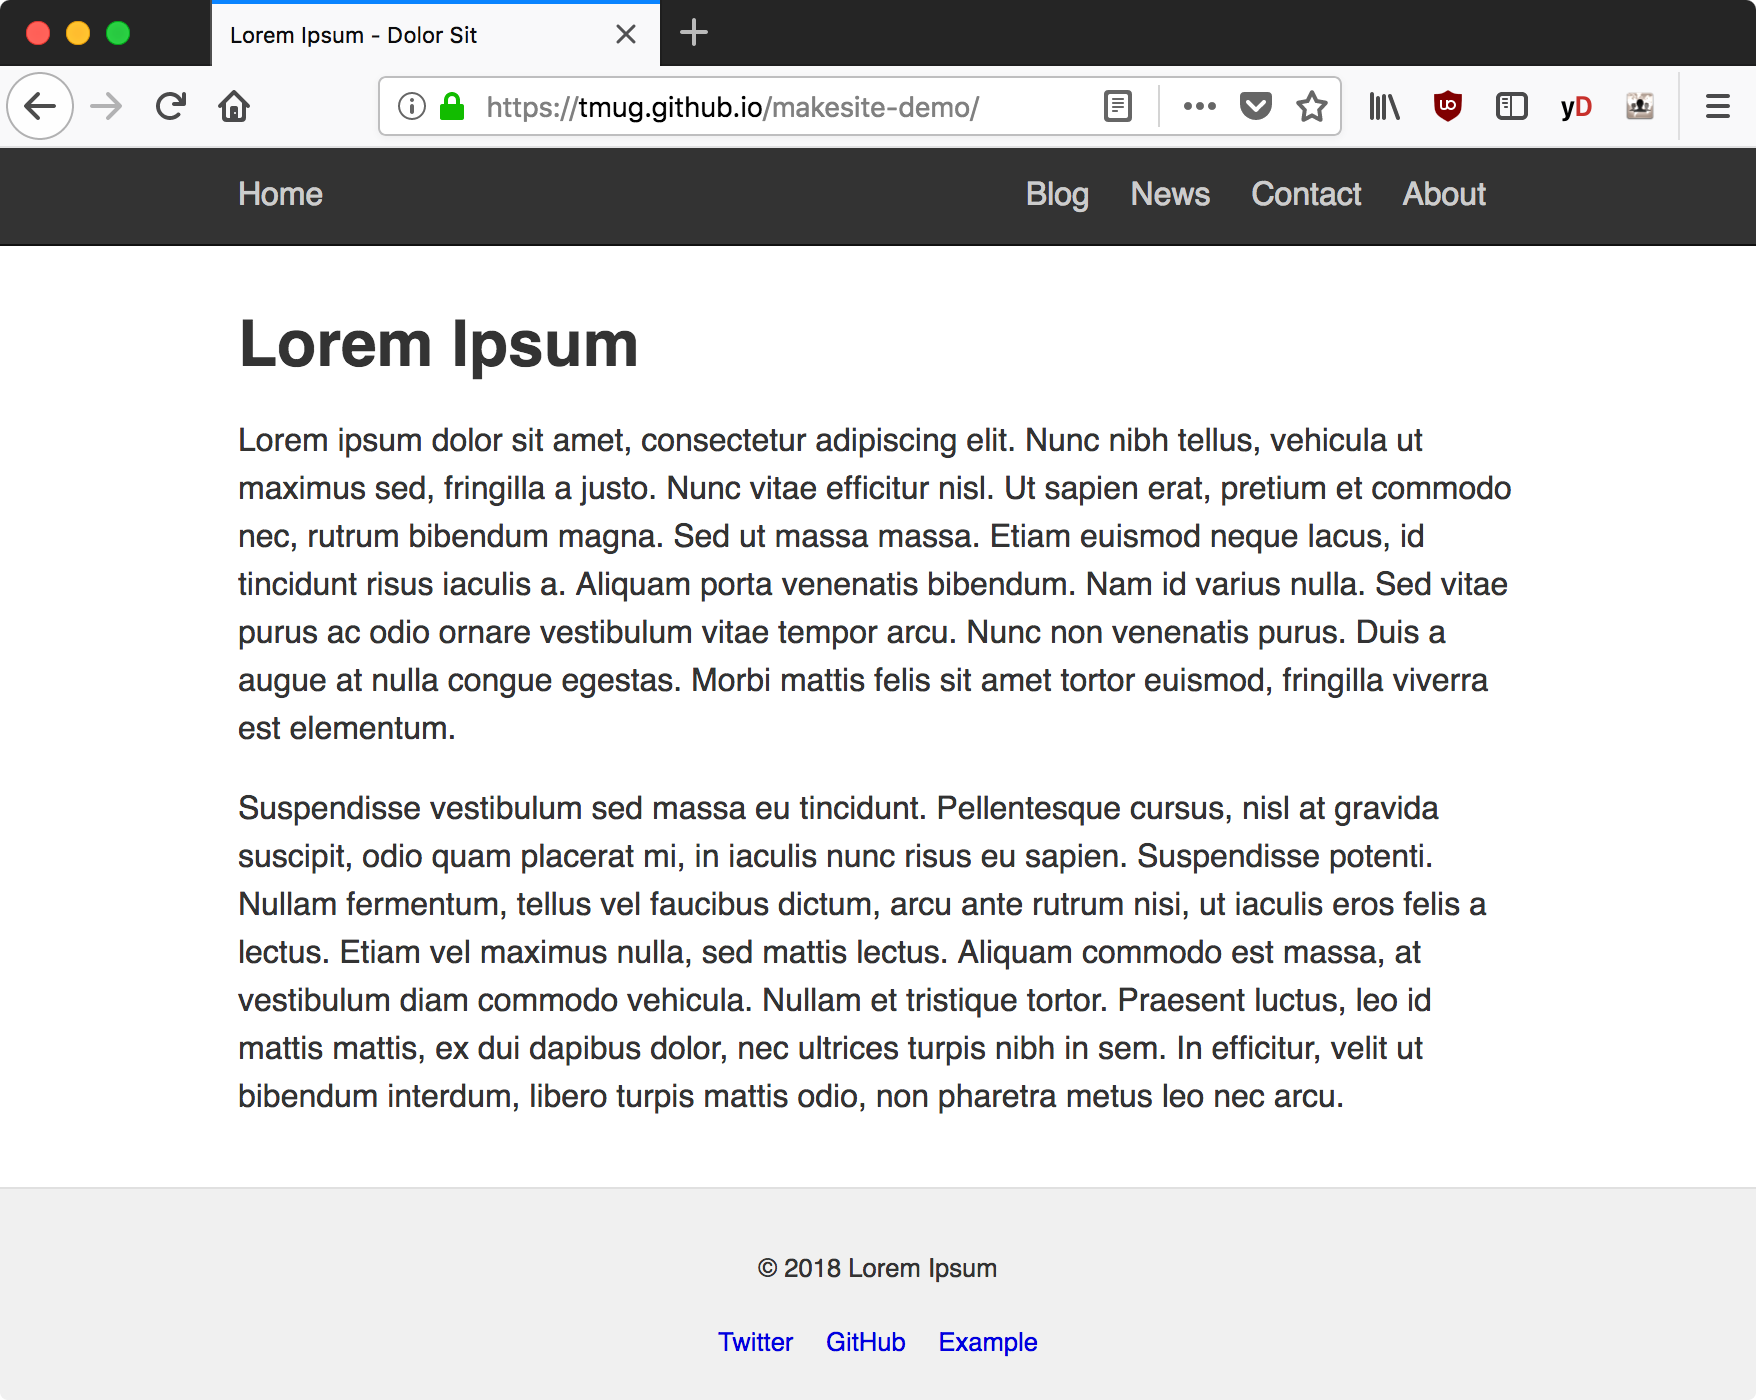
\includegraphics[height=2.4in]{makesite-demo-home.png}
        \caption{Screenshot of demo static website generated with makesite.py}
    \end{figure}

    \linkcaption{
        Demo website: \url{https://tmug.github.io/makesite-demo/}
    }
\end{frame}


% Demo Static Blog (Screenshot)
\begin{frame}
    \frametitle{Demo Static Blog}

    \begin{figure}
        \centering
        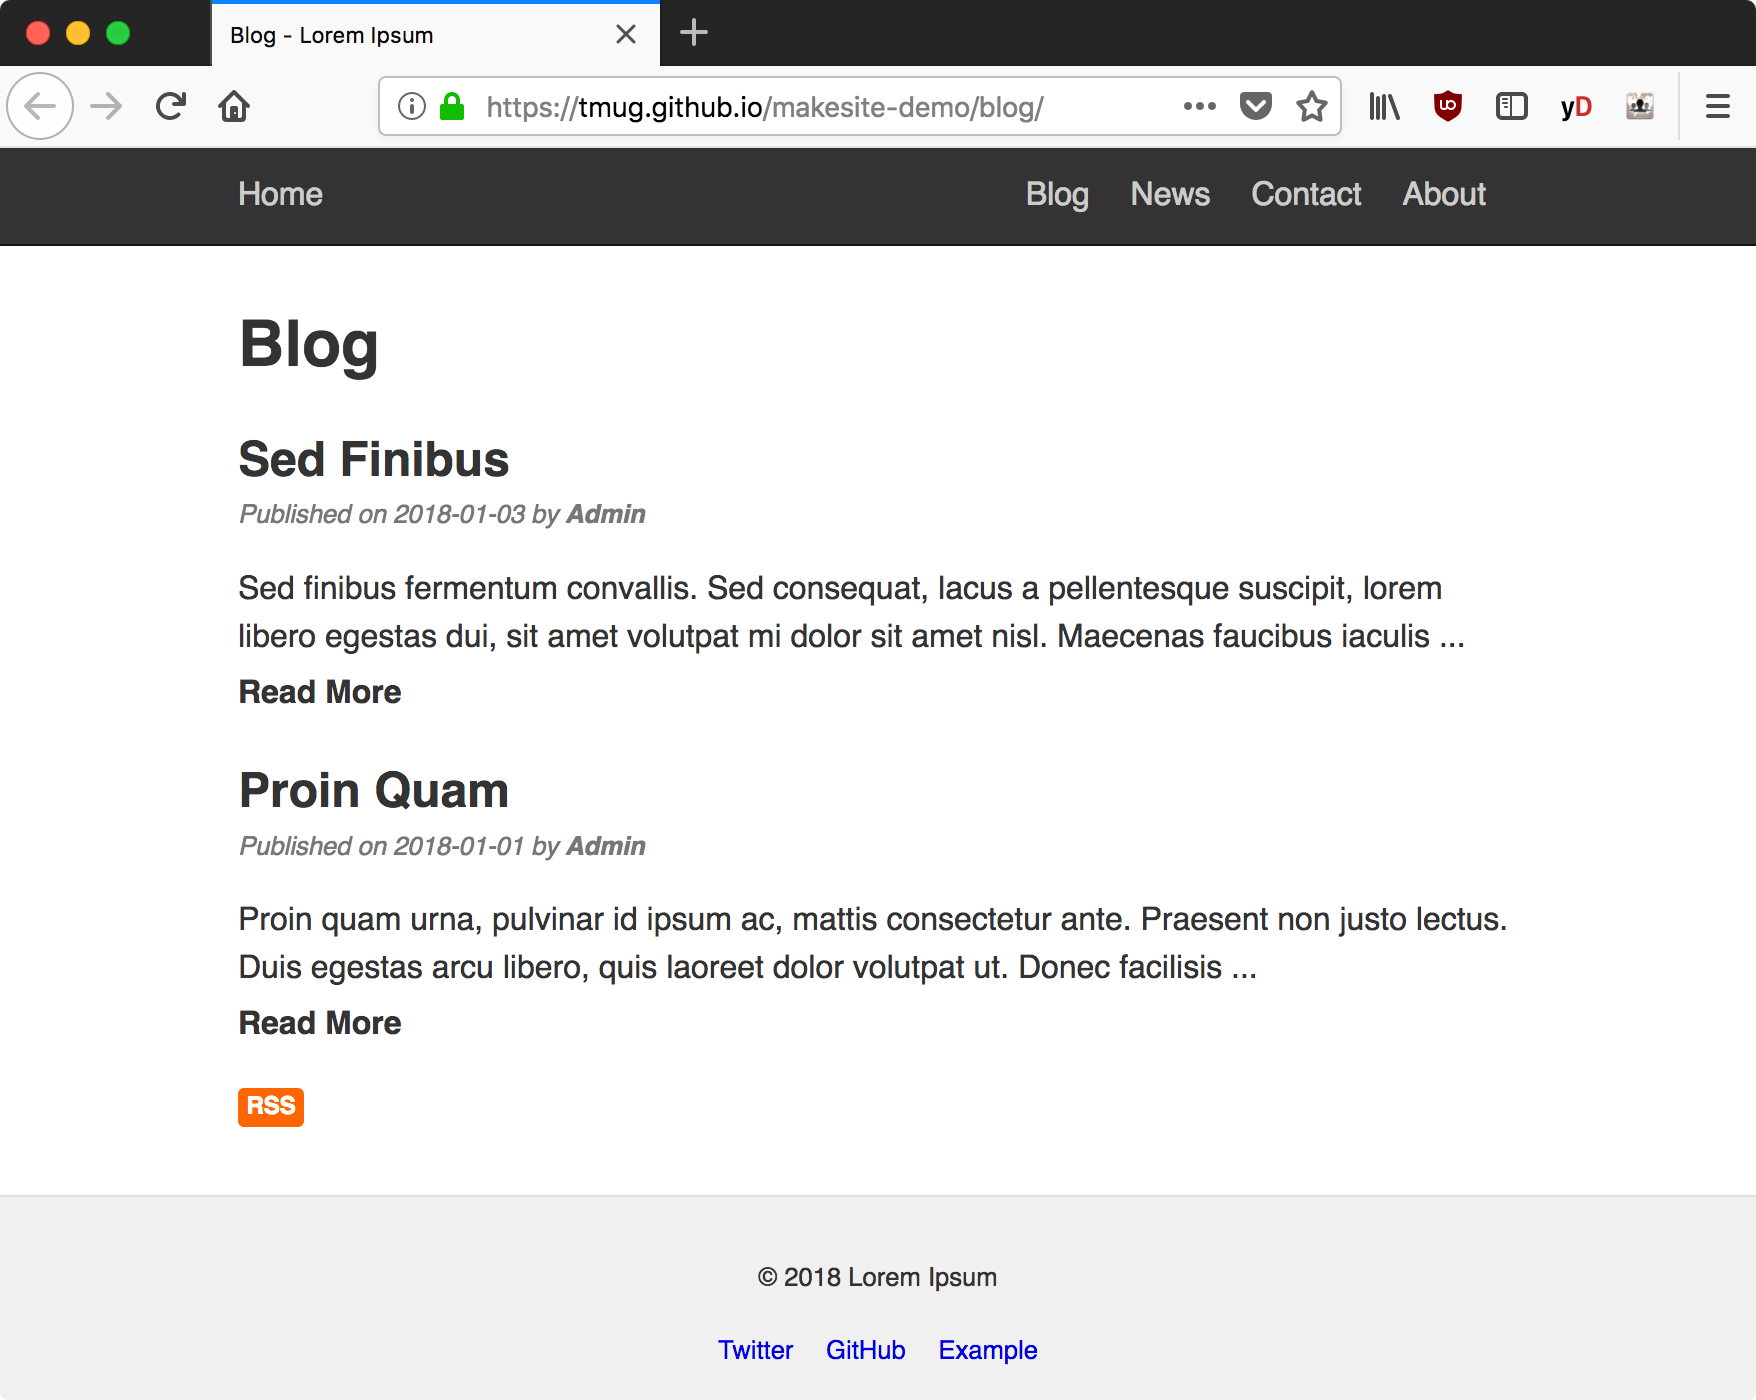
\includegraphics[height=2.4in]{makesite-demo-blog.png}
        \caption{
            Screenshot of demo static blog generated with makesite.py
        }
    \end{figure}

    \linkcaption{
        Demo blog: \url{https://tmug.github.io/makesite-demo/blog/}
    }
\end{frame}


% On Show HN Page (Screenshot)
\begin{frame}
    \frametitle{On ``Show HN'' Page}

    \begin{figure}
        \centering
        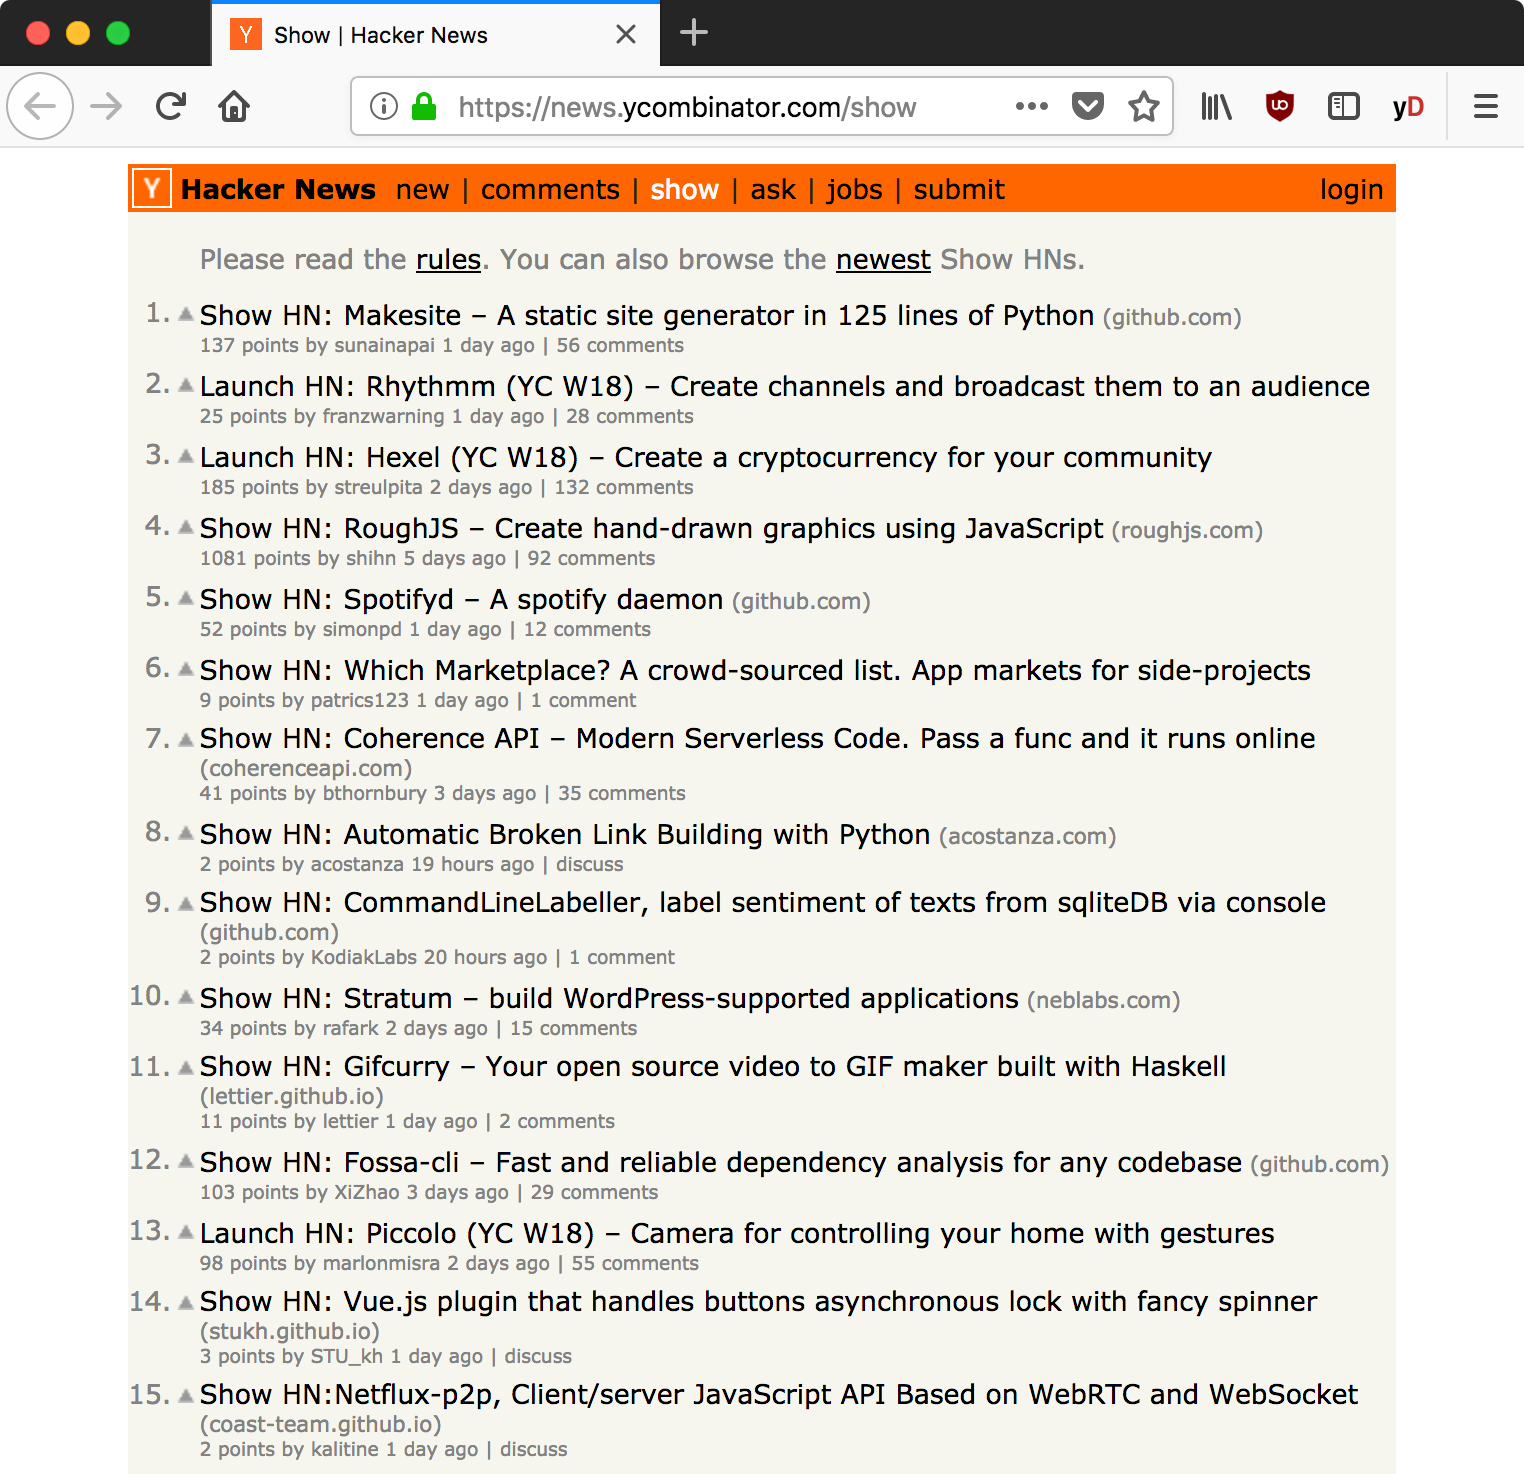
\includegraphics[height=2.4in]{makesite-showhn.png}
        \caption{
            Makesite trending at the top of the ``Show HN`` posts on
            18 Mar 2018
        }
    \end{figure}

    \linkcaption{
        Hacker News ``Show HN'' story:
        \url{https://news.ycombinator.com/item?id=16606408}
    }

    \begin{tikzpicture}[remember picture, overlay]
        \node [xshift=35.4mm, yshift=67.5mm] at (current page.south west) {
            \footnotesize \faHandORight
        };
    \end{tikzpicture}
\end{frame}


% On GitHub Trending Page (Screenshot)
\begin{frame}
    \frametitle{On GitHub Trending Page}

    \begin{figure}
        \centering
        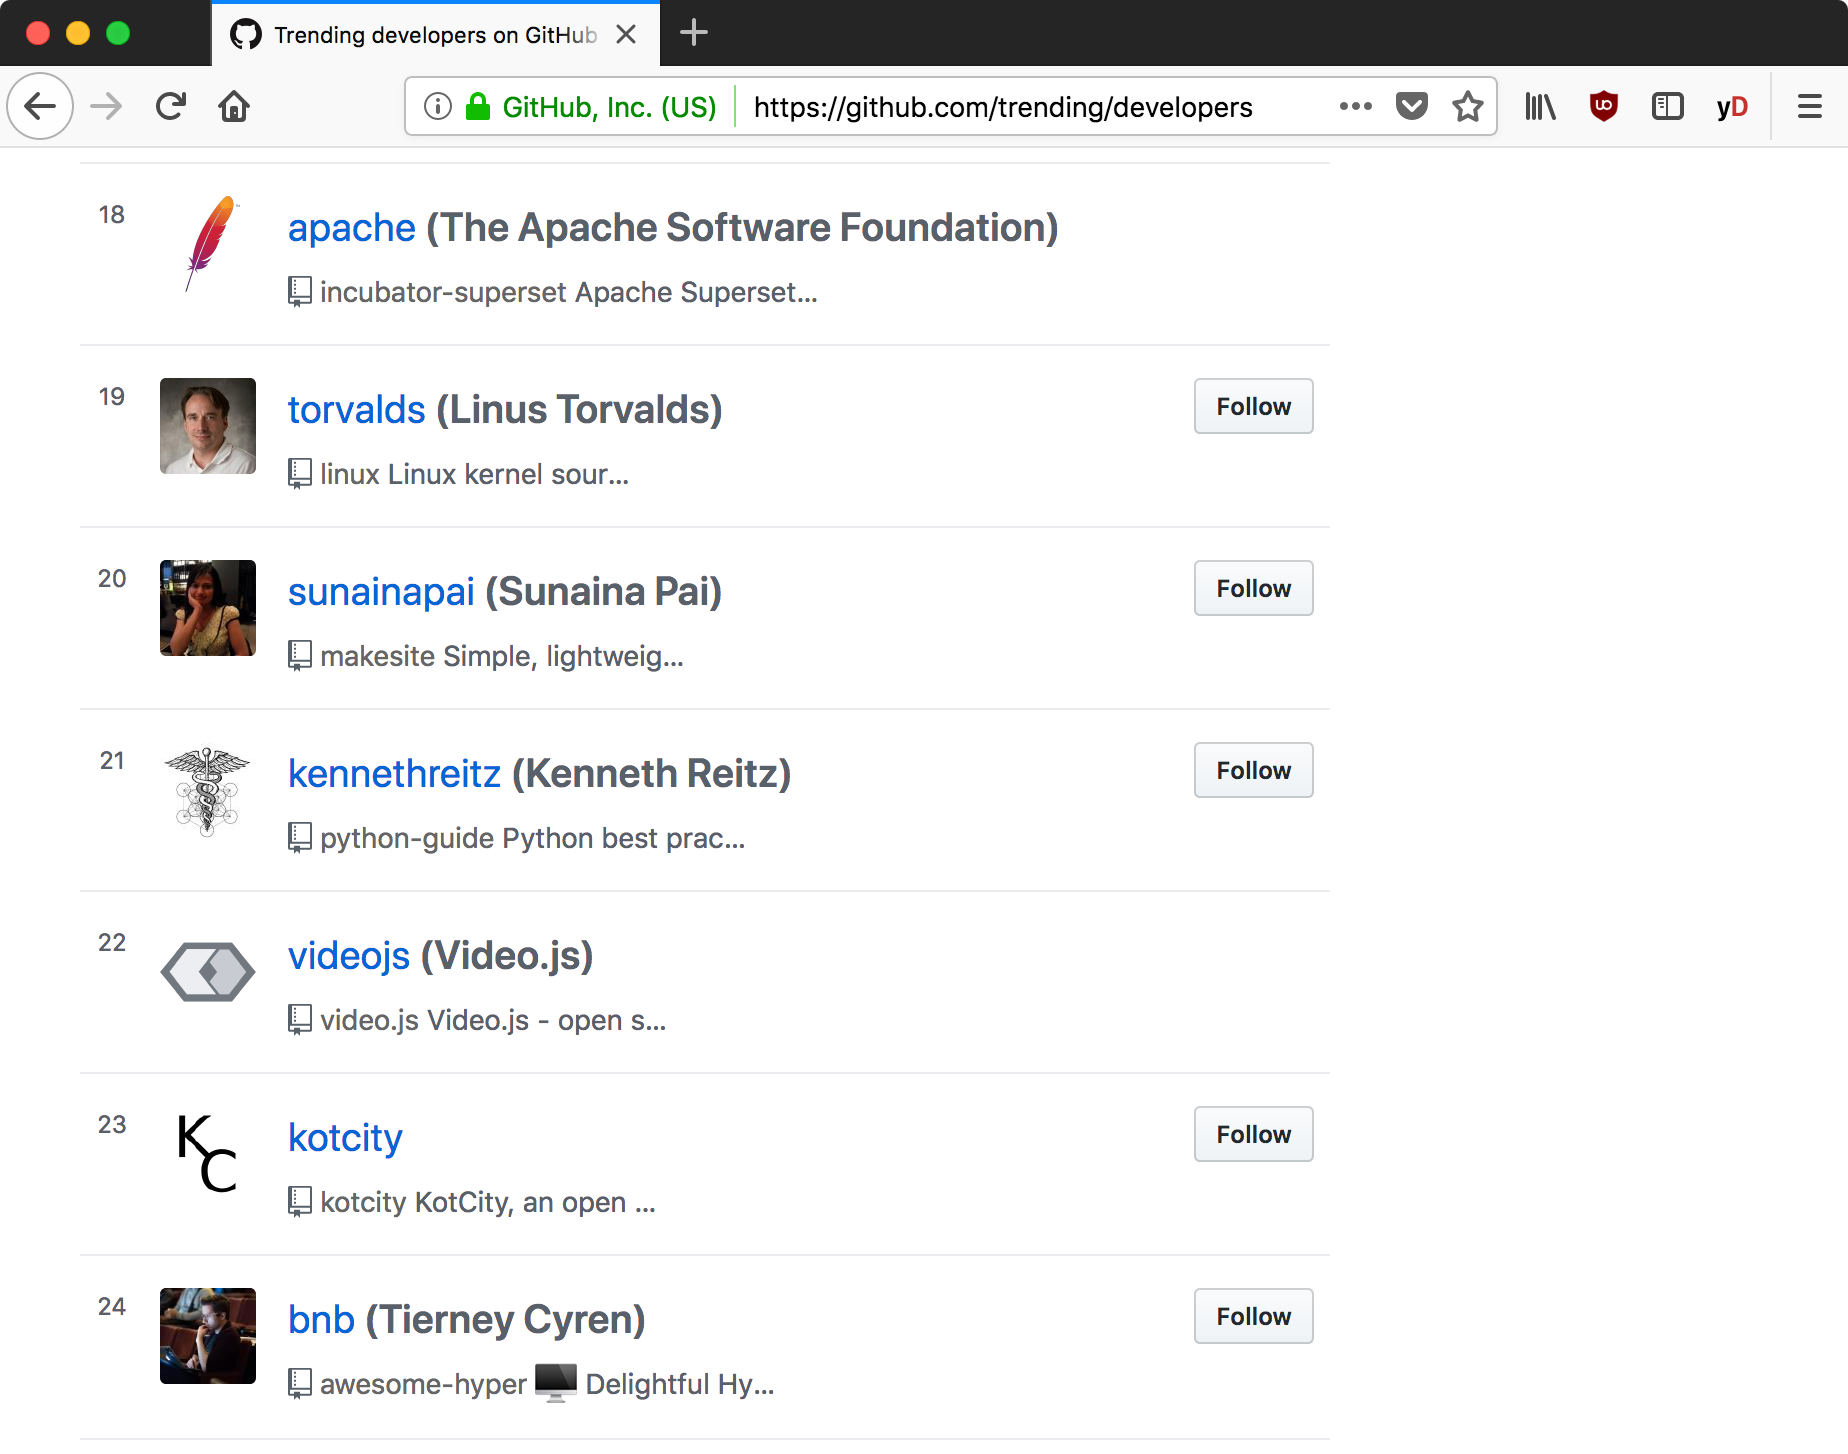
\includegraphics[height=2.7in]{sunaina-trending.png}
        \caption{
            Nice to be trending up there with Linus Torvalds!
            \raisebox{-0.3em}{
                
\includegraphics[width=1.5em]{cheeky.png}
            }
        }
    \end{figure}

\end{frame}


% Summary
\begin{frame}
    \frametitle{Summary of Work}
    \begin{itemize}
        \item Write code.
        \item Write unit tests.
        \item Write README.
        \item Publish on GitHub.
        \item Integrate with Travis CI and Coveralls.
        \item Set up an online demo.
        \item Announce on Hacker News.
    \end{itemize}
\end{frame}


% Results
\begin{frame}
    \frametitle{Results}
    \begin{itemize}
        \item Got a small community of Python developers who use the project.
        \item Received pull requests to improve the software.
        \item Became a part of a very welcoming community.
    \end{itemize}
\end{frame}


% Thank You.
\begin{frame}
    \begin{center}
        \Huge
        Thank You!
    \end{center}
\end{frame}

\end{document}
